\documentclass[aspectratio=169]{beamer}

\setbeamersize{text margin left=5mm, text margin right=5mm}

\defbeamertemplate{headline}{my header}{%
\vskip1pt%
\makebox[0pt][l]{\,\insertshortauthor}%
\hspace*{\fill}\insertshorttitle/\insertshortsubtitle\hspace*{\fill}%
\llap{\insertpagenumber/\insertpresentationendpage\,}
}
\setbeamertemplate{headline}[my header]

\let\olditem\item
\renewcommand{\item}{\setlength{\itemsep}{\fill}\olditem}

\usepackage{bm}
\usepackage{graphicx}
\usepackage{caption}
\usepackage{soul}
\usepackage{tkz-euclide}
\usetikzlibrary{calc}
\usepackage[]{algorithm2e}
\usepackage{changepage}
\usepackage{amssymb}
\usepackage{xcolor}
\usepackage{mathtools}
\usepackage{tcolorbox}
\usepackage{tikz}
\usepackage{tikz-3dplot}
\usepackage{tkz-euclide}
\usepackage{pgfplots}
\pgfplotsset{width=5cm,compat=1.3}
\usepackage{circuitikz}
\usepackage{mleftright}
% \usepackage{algorithm,algorithmic}
\usetikzlibrary{arrows.meta, decorations.pathreplacing, positioning, shapes.geometric}
\usetikzlibrary{arrows}

\usepackage{pgfplots}
\usetikzlibrary{plotmarks}
\pgfplotsset{width=7cm,compat=1.8}
\pgfplotsset{compat=1.17}

\usetikzlibrary{positioning}
% \usepackage[math]{cellspace}
% \cellspacetoplimit 4pt
% \cellspacebottomlimit 4pt
%\usetikzlibrary{arrows.meta}
% sqare of half axes
\newcommand{\asa}{3}
\newcommand{\bsa}{1}
\newcommand{\csa}{0.25}
% view angle
\tdplotsetmaincoords{70}{135}


%% Fonts
\usefonttheme{professionalfonts}
\usefonttheme{serif}

\DeclareCaptionLabelFormat{blank}{}
\captionsetup[figure]{labelformat=blank}

%% Math definitions
\def\mf{\ensuremath\mathbf}
\def\mb{\ensuremath\mathbb}
\def\mc{\ensuremath\mathcal}
\def\lp{\ensuremath\left(}
\def\rp{\ensuremath\right)}
\def\lv{\ensuremath\left\lvert}
\def\rv{\ensuremath\right\rvert}
\def\lV{\ensuremath\left\lVert}
\def\rV{\ensuremath\right\rVert}
\def\lc{\ensuremath\left\{}
\def\rc{\ensuremath\right\}}
\def\ls{\ensuremath\left[}
\def\rs{\ensuremath\right]}
\def\bmx{\ensuremath\begin{bmatrix*}[r]}
\def\emx{\ensuremath\end{bmatrix*}}
\def\bmxc{\ensuremath\begin{bmatrix*}[c]}
\def\R{\ensuremath\mb{R}}
\def\t{\lp t\rp}
\def\k{\ls k\rs}

\newcommand{\demoex}[2]{\onslide<#1->\begin{color}{black!60} #2 \end{color}}
\newcommand{\demoexc}[3]{\onslide<#1->\begin{color}{#2} #3 \end{color}}
\newcommand{\anim}[3]{\onslide<#1->{\begin{color}{#2!60} #3 \end{color}}}
\newcommand{\ct}[1]{\lp #1\rp}
\newcommand{\dt}[1]{\ls #1\rs}
\newcommand{\cols}[2]{\begin{columns}[#1] #2 \end{columns}}
\newcommand{\col}[2]{\begin{column}{#1} #2 \end{column}}

%% Mycolors
\definecolor{myred}{RGB}{192,0,0}
\definecolor{mygray}{RGB}{100,100,100}

%% Custom beamer color
\setbeamercolor{title}{fg=myred}
\setbeamercolor{subtitle}{fg=myred}
\setbeamerfont{title}{series=\bfseries}
% \setbeamercolor{frametitle}{bg=myred, fg=white}
\setbeamercolor{frametitle}{bg=mygray!10!, fg=myred}
\setbeamerfont{frametitle}{series=\bfseries}
\setbeamercolor{item}{fg=mygray}
\setbeamercolor{title in head/foot}{fg=myred}

% Move header to footer
\setbeamertemplate{headline}{}
\setbeamertemplate{footline}{
  \begin{beamercolorbox}[wd=\paperwidth,ht=2.25ex,dp=1ex,center]{footline}
    \inserttitle\hfill\insertauthor\hfill\insertdate\hfill\insertframenumber{}
  \end{beamercolorbox}
}

\pgfplotsset{
colormap={whitered}{color(0cm)=(white); color(1cm)=(orange!75!red)}
}


\title{Applied Linear Algebra in Data Analysis}

% A subtitle is optional and this may be deleted
\subtitle{Introduction to Optimization}

\author{Sivakumar Balasubramanian}
% - Give the names in the same order as the appear in the paper.
% - Use the \inst{?} command only if the authors have different
%   affiliation.

\institute[Christian Medical College] % (optional, but mostly needed)
{
  \inst{}%
  Department of Bioengineering\\
  Christian Medical College, Bagayam\\
  Vellore 632002
}
% - Use the \inst command only if there are several affiliations.
% - Keep it simple, no one is interested in your street address.

\date{}
% - Either use conference name or its abbreviation.
% - Not really informative to the audience, more for people (including
%   yourself) who are reading the slides online

\subject{Lecture notes on ALADA}
% This is only inserted into the PDF information catalog. Can be left
% out. 

% If you have a file called "university-logo-filename.xxx", where xxx
% is a graphic format that can be processed by latex or pdflatex,
% resp., then you can add a logo as follows:

% \pgfdeclareimage[height=0.5cm]{university-logo}{university-logo-filename}
% \logo{\pgfuseimage{university-logo}}

% Delete this, if you do not want the table of contents to pop up at
% the beginning of each subsection:
\AtBeginSubsection[]
{
  \begin{frame}<beamer>{Outline}
    \tableofcontents[currentsection,currentsubsection]
  \end{frame}
}

% Let's get started
\begin{document}

\pgfplotsset{
  compat=1.8,
  colormap={whitered}{color(0cm)=(white); color(1cm)=(orange!75!red)}
}


\begin{frame}
  \titlepage
\end{frame}


\begin{frame}[t]{Optimization}
\begin{itemize}
  \item Optimization is the process of finding the best solution to a problem from a set of possible solutions.
  \item Optimization problems come up in many applications in engineering, science, economics, biology, medicine, operations research, etc.
  \item Optimization problems can be classified in different ways, but one major classification gives us: \textbf{unconstrained} and \textbf{constrained} optimization problems.
\end{itemize}
\end{frame}


\begin{frame}[t]{A general optimization problem}
\begin{itemize}
  \item A general optimization problem can be fomulated as the following,
  \[ \begin{split}
      \min_{\mf{x}} & \,\,\, f\ct{\mf{x}} \\
      \mathrm{subject \,\, to} & \,\,\, \mf{g}\ct{\mf{x}} \leq \mf{0}, \,\, \mf{g}\ct{\mf{x}} = \bmx g_1\ct{\mf{x}} & g_2\ct{\mf{x}} & \cdots & g_p\ct{\mf{x}}\emx^\top \\
      & \,\,\, \mf{h}\ct{\mf{x}} = \mf{0}, \,\, \mf{h}\ct{\mf{x}} = \bmx h_1\ct{\mf{x}} & h_2\ct{\mf{x}} & \cdots & h_q\ct{\mf{x}}\emx^\top \\
  \end{split} \]
  where, $f\ct{\mf{x}}$ is the \textbf{objective function} and $\mf{g}\ct{\mf{x}}$ represents the set of \textbf{inquality constaints} and $\mf{h}\ct{\mf{x}}$ represents the set of \textbf{equality constraints}.

  \item In this course, we will only focus on optimization problems over $\R^n$, and mostly problems where the objective function and the constraints are differentiable.
\end{itemize}
\end{frame}


\begin{frame}[t]{A general optimization problem}
\begin{itemize}
  \item Most optimization problems of practical significance cannot be solved analytically, and we must resort to numerical iterative methods to find a solution.
  
  \item We can never solve these problems exactly through numerical means, and must content outselves with finding an approximate ``good enough'' solution.
\end{itemize}
\end{frame}


\begin{frame}[t]{Mathematical preliminaries: Sequences and Limits}
  We first review the notions of continuity and differentiability of functions of single and multiple variables, since we will be dealing with differentiable functions in optimization problems.
  \vspace{0.2cm}

  \textbf{Sequences and Limits}:
  \begin{itemize}
    \item A \text{sequence of real numbers} is a function whose domain is a set of natural numbers $1, 2, \ldots, k, \ldots$ and whose range is a set of real numbers. The sequence is denoted by $\lc x_k\rc_{k=1}^{\infty}$ or $\lc x_k \rc$.
    \vspace{0.25cm}
  
    \item A number $x^{*}$ is said to be the \textbf{limit} of the sequence $\lc x_k \rc$ if for every $\epsilon > 0$, there exists an integer $K$ such that for all $k > K$, we have $\lv x_k - x^{*} \rv < \epsilon$.
    \[ \lim_{k \to \infty} x_k = x^* \quad \mathrm{or} \quad x_k \to x^* \]

    A sequence that has a limit is called a \textbf{convergent sequence}.
  \end{itemize}
\end{frame}


\begin{frame}[t]{Sequences and Limits}
  We can extend these ideas to $\R^n$.
  \begin{itemize}
    \item A sequence in $\R^n$ is a function whose domain is a set of natural numbers $1, 2, \ldots, k, \ldots$ and whose range is $\R^n$. The sequence is denoted by $\lc \mf{x}_k\rc_{k=1}^{\infty}$ or $\lc \mf{x}_k \rc$.
    \vspace{0.25cm}
  
    \item $\mf{x}^{*}$ is said to be the \textbf{limit} of the sequence $\lc \mf{x}_k \rc$ if for every $\epsilon > 0$, there exists an integer $K$ such that for all $k > K$, we have $\lV \mf{x}_k - \mf{x}^{*} \rV < \epsilon$.
    \[ \lim_{k \to \infty} \mf{x}_k = \mf{x}^* \quad \mathrm{or} \quad \mf{x}_k \to \mf{x}^* \]

    \item The limit of a convergent sequence is unique.
  \end{itemize}
\end{frame}


\begin{frame}[t]{Continuity}
  Consider the function $f: \Omega \to \R$, where $\Omega \subseteq \R^n$. This function is continuous at the point $\mf{x}_0 \in \Omega$, if and only if, 
  \[ \lim_{\mf{x} \to \mf{x}_0} f\ct{\mf{x}} = f\ct{\mf{x}_0} \]
  
  \begin{figure}
    \centering
    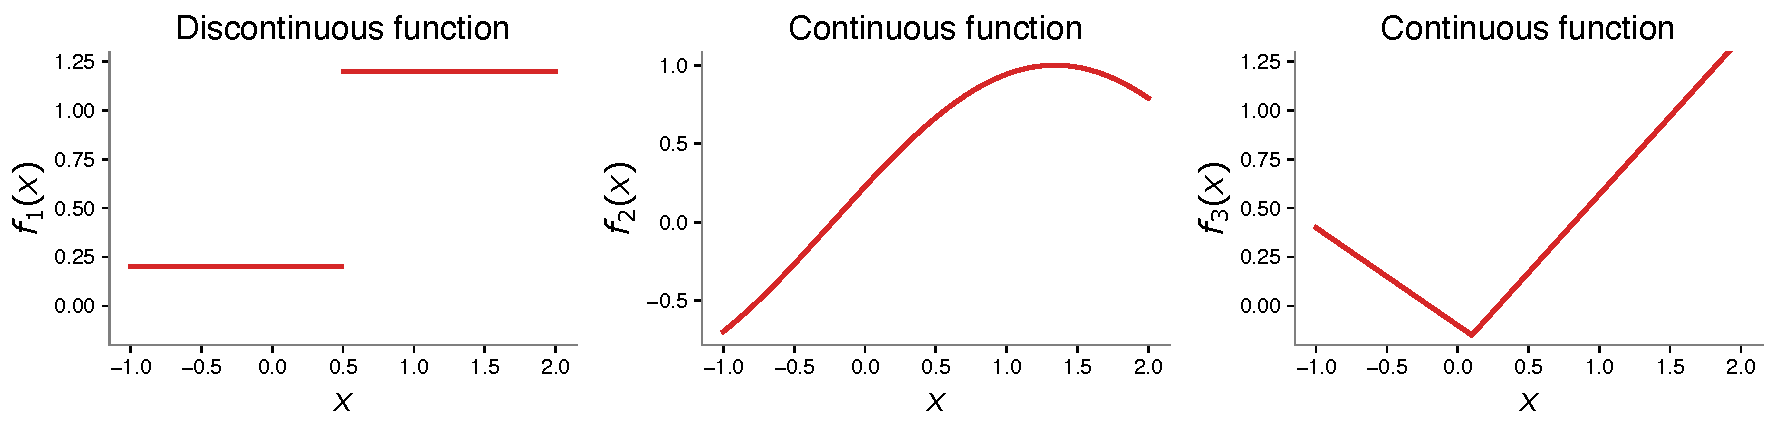
\includegraphics[width=\textwidth]{figs/func_cont.pdf}
  \end{figure}
\end{frame}


\begin{frame}[t]{Differentiability}
  Differentiability is a local property of a function, like continuity. 
  
  Consider a function $f: \Omega \to \R$, where $\Omega \subseteq \R$. Let $x_0 \in \Omega$,
  \[ \frac{\delta f\ct{x_0}}{\delta x} = \frac{f\ct{x_0 + \delta x} - f\ct{x_0}}{\delta x} \]

  The function $f$ is said to be differentiable at the point $x_0 \in \Omega$, if and only if,
  \begin{itemize}
    \item $f\ct{x}$ is continuous at $x_0$.
    \item $\lim_{\delta x \to 0} \frac{\delta f\ct{x_0}}{\delta x} = \lim_{\delta x \to 0^-}\frac{\delta f\ct{x_0}}{\delta x}  = \lim_{\delta x \to 0^+} \frac{\delta f\ct{x_0}}{\delta x}$
    \item $\lim_{\delta x \to 0} \frac{f\ct{x_0}}{\delta x}$ is finite.
  \end{itemize}

  Then the derivative of the function  $f$ at the point $x_0$ is defined as,
  \[ \frac{df\ct{x_0}}{dx} = \lim_{\delta x \to 0} \frac{f\ct{x_0 + \delta x} - f\ct{x_0}}{\delta x} \]
\end{frame}


\begin{frame}[t]{Differentiability}
  Three functions $f_1, f_2, f_3$ defined over the set $\Omega = \left[ -1, 2\right] \subseteq \R$.
  
  \begin{figure}
    \centering
    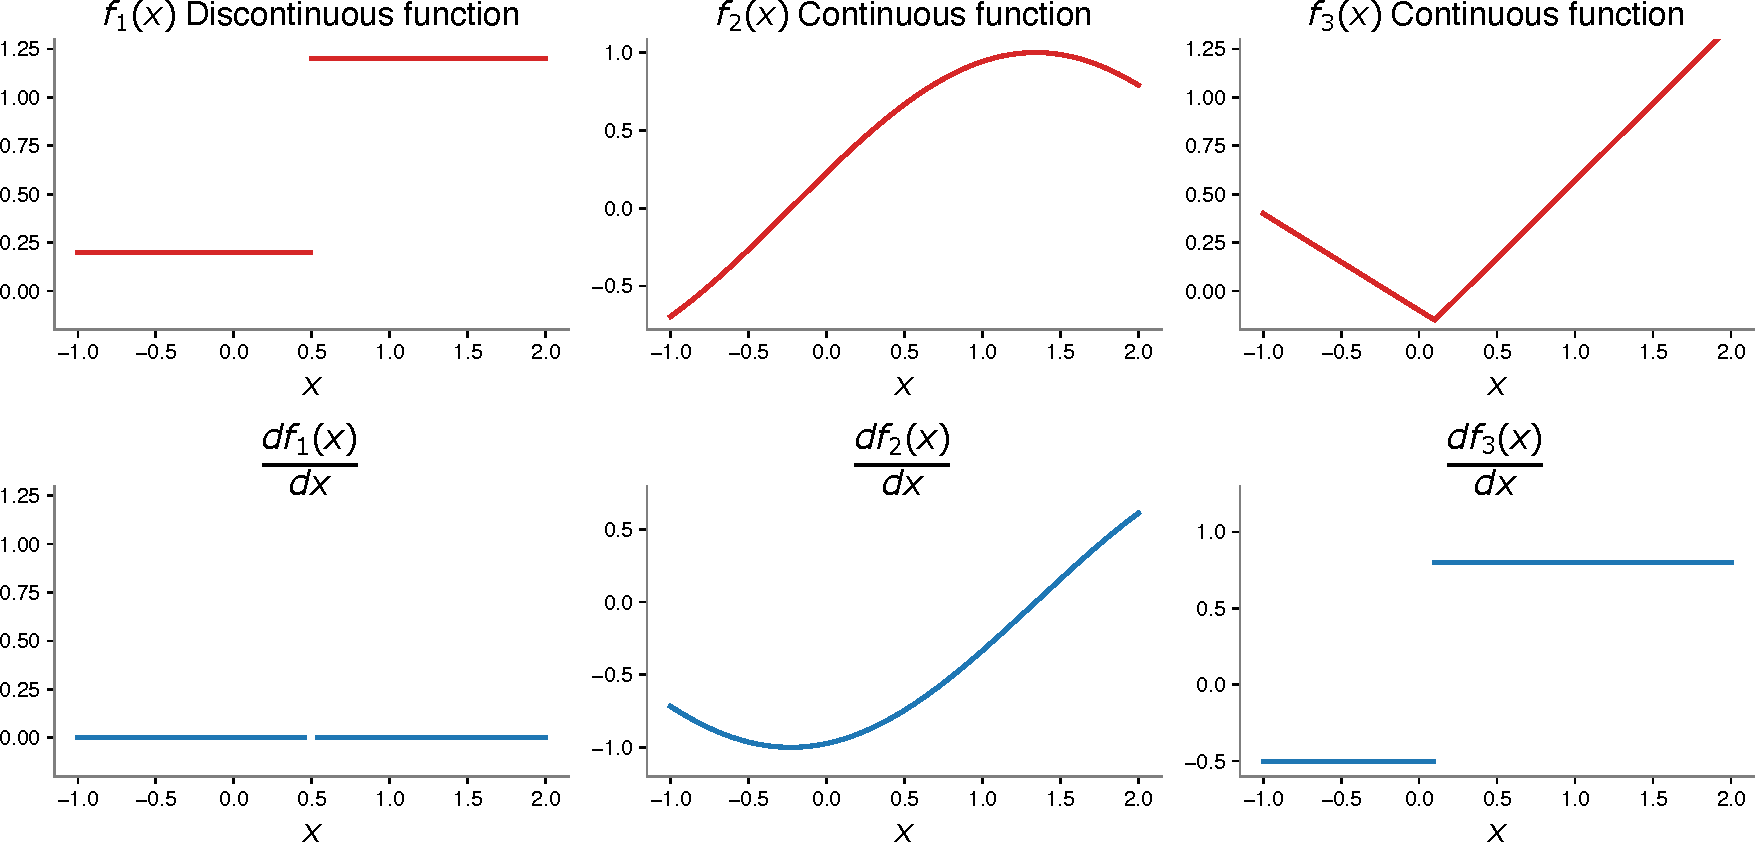
\includegraphics[width=0.85\textwidth]{figs/func_diff.pdf}
  \end{figure}
\end{frame}


\begin{frame}[t]{Differentiability in $\R^n$}
  Consider the function $f: \Omega \to \R$, where $\Omega \subseteq \R^n$.
  \[ f\ct{\mf{x}} = f\ct{x_1, x_2, \ldots, x_n} \]
  $f$ maps a column vector $\mf{x} = \bmx x_1 & x_2 & \cdots & x_n \emx^\top \in \mb{R}^n$ to a real number.
  \vspace{0.25cm}

  The partial derivative of the function $f\ct{\mf{x}}$ at $\mf{x}_0$ is defined as,
  \[ \frac{\partial f\ct{\mf{x}_0}}{\partial x_i} = \lim_{\delta x \to 0} \frac{f\ct{\mf{x}_0 + \delta x \, \mf{e}_i} - f\ct{\mf{x}_0}}{\delta x} \]

  $\frac{\partial f\ct{\mf{x}}}{\partial x_i}$ is the rate of change of the function $f$ when move along the $i$-th coordinate direction at the point $\mf{x}_0$.
  \vspace{0.25cm}
  
  The function $f$ is said to be differentiable at the point $\mf{x}_0 \in \Omega$, if and only if, the partial derivatives of the function $f$ w.r.t. all $x_i$ exist.
\end{frame}


\begin{frame}[t]{Differentiability in $\R^n$}
  The derivative of the function $f: \Omega \to \R$, where $\Omega \subseteq \R^n$ with respect to the column vector $\mf{x}$ at the point $\mf{x}_0 \in \Omega$ is defined as the following,
  \[ \nabla f\ct{\mf{x}_0} = \bmx \frac{\partial f}{\partial x_1}\ct{\mf{x}_0} & \frac{\partial f}{\partial x_2}\ct{\mf{x}_0} & \cdots & \frac{\partial f}{\partial x_n}\ct{\mf{x}_0}\emx \in \mb{R}^n \]
  Notice that $\nabla f\ct{\mf{x}_0}$ is a row vector, and it is called the \textit{gradient} of the function $f$ at the point $\mf{x}_0$.

  We follow the following convention when dealing with derivative of functions of multiple variables $f: \Omega \to \R$:
  \begin{itemize}
    \item The gradient with respect to a column vector $\mf{x}$ is a row vector $\nabla_{\mf{x}} f\ct{\mf{x}}$.
    \[ \nabla_{\mf{x}} f\ct{\mf{x}} = \bmx \frac{\partial f}{\partial x_1} & \frac{\partial f}{\partial x_2} & \cdots & \frac{\partial f}{\partial x_n} \emx \]
    \item The gradient with respect to a row vector $\mf{x}^\top$ is a column vector $\nabla_{\mf{x}^\top} f\ct{\mf{x}}$.
    \[ \nabla_{\mf{x}^\top} f\ct{\mf{x}} = \bmx \frac{\partial f}{\partial x_1} & \frac{\partial f}{\partial x_2} & \cdots & \frac{\partial f}{\partial x_n} \emx^\top \]
  \end{itemize}
\end{frame}


\begin{frame}[t]{Differentiability in $\R^n$: Jacobian of a Vector-valued function}
  Consider the function $\mf{h}: \R^q \to \R^p$, where
  \[ \mf{h}\ct{\mf{x}} = \bmx h_1\ct{\mf{x}} & h_2\ct{\mf{x}} & \cdots & h_p\ct{\mf{x}} \emx^\top \,\,\, \mf{x} \in \R^q \]

  The \textit{Jacobian} of the function $\mf{h}\ct{\mf{x}}$ with respect to $\mf{x} \in \R^q$ is defined as the following matrix,
  \[ \nabla_{\mf{x}} \mf{h}\ct{\mf{x}} \triangleq \bmxc \nabla_{\mf{x}} h_1\ct{\mf{x}} \\ \nabla_{\mf{x}} h_2\ct{\mf{x}} \\ \vdots \\ \nabla_{\mf{x}} h_p\ct{\mf{x}}\emx \in \R^{p \times q}\]
\end{frame}


\begin{frame}[t]{Differentiability in $\R^n$: Hessian Matrices}
  Consider the function $f: \R^n \to \R$ and $\mf{x} \in \R^n$. 
  \vspace{0.25cm}

  The Hessian matrix $\mf{H}_f\ct{\mf{x}}$ of the function $f\ct{\mf{x}}$  is defined as the symmetric matrix $n \times n$ matrix of the second order partial derivatives of $f$ with respect to the components of $\mf{x}$, assuming all the second order partial derivatives exists.
  \vspace{0.25cm}

  The $ij^{th}$ element of the Hessian matrix of $f\ct{\mf{x}}$ is given by.
  \[ \ls \mf{H}_f\ct{\mf{x}}\rs_{ij} = \frac{\partial^2 f}{\partial x_i \partial x_j}\ct{\mf{x}} = \frac{\partial}{\partial x_i}\ct{\frac{\partial f}{\partial x_j}\ct{\mf{x}}} = \frac{\partial}{\partial x_j}\ct{\frac{\partial f}{\partial x_i}\ct{\mf{x}}} \]
  % \vspace{0.25cm}

  \[ \mf{H}_f\ct{\mf{x}} \triangleq \bmxc \frac{\partial^2 f}{\partial x_1^2} & \cdots & \frac{\partial^2 f}{\partial x_1 \partial x_n} \\
  \vdots & \ddots & \vdots \\
  \frac{\partial^2 f}{\partial x_n \partial x_1} & \cdots & \frac{\partial^2 f}{\partial x_n^2} \emx \quad \mf{H}_f\ct{\mf{x}} = \nabla_{\mf{x}^\top}\ct{\nabla_{\mf{x}} f\ct{\mf{x}}} = \nabla_{\mf{x}}\ct{\nabla_{\mf{x}^\top} f\ct{\mf{x}}} \]
\end{frame}


\begin{frame}{Gradient of a function $f: \R^n \to \R$}
  The levels set of the function $f: \R^n \to \R$ at the level $c \in \R$ is defined as,
  \[ S = \lc \mf{x} \,\, \mid \,\, \mf{x} \in \R^n. \, f\ct{\mf{x}} = c\rc \] 
  A level set is a curve for functions $f: \R^2 \to \R$, and is a surface when $f: \R^3 \to \R$.
  \vspace{0.25cm}

  The different level sets are also called the contours of the function $f$.
  \vspace{0.25cm}

  The gradient of the function $f$ at a point $\mf{x}_0$ is orthogonal to the level set of the function $f$ at the value $f\ct{\mf{x}_0}$.
  \vspace{0.25cm}

  The gradient is also the direction in $\R^n$ of maximal increase of the value of the function $f$. This is also called the direction of \textit{steepest ascent}.
\end{frame}


\begin{frame}{Taylor's Theorem}
  Many results from analysis are used in optimization problems --  one of them is the ``Taylor's'' theorem.

  The Taylor's theorem gives an polynomial approximation of a $k$ time differentiaable function $f: \R \to \R$ around at a given point $x_0$ by a $k^{th}$ order \textbf{Taylor polynomial}.

  For a smooth function (infinitely differentiable), the $k^{th}$ order Taylor polynomial is a truncation at the order $k$ of the Taylor series expansion of the function $f$ around the point $x_0$.

  \textbf{Taylor's Theoerem}: Suppose a function $f: \R \to \R$ is $k$ times differentiable at a point $x_0$, then the function $f$ can be approximated by the following polynomial with $\epsilon = x - x_0$,
  \[ f\ct{x} = f\ct{x_0} + Df\ct{x_0} \frac{\epsilon}{1!} + D^2f\ct{x_0} \frac{\epsilon^2}{2!} + \cdots + D^{k-1}f\ct{x_0}\frac{\epsilon^{k-1}}{\ct{k-1}!} + D^{k}f\ct{x_0 + \theta \epsilon}\frac{\epsilon^{k}}{\ct{k}!} \]
  where, $D^l f\ct{x_0}$ is the $l^{th}$ order derivative of the function $f$ at the point $x_0$, and $0 \leq \theta \leq 1$ .
\end{frame}


\begin{frame}{Taylor's Theorem}
  Now consider a function $f: \R^n \to \R$ and $\mf{x}_0 \in \R^n$, and let's assume that $f$ is differentiable twice with respect to $\mf{x}$, and let $\bm{\epsilon} = \mf{x} - \mf{x}_0$. The polynomial approximation of $f$ is given by,
  \[ f\ct{\mf{x}} = f\ct{\mf{x}_0} + \frac{1}{1!}\mf{g}\ct{\mf{x}_0}^\top \bm{\epsilon} +  \frac{1}{2!} \bm{\epsilon}^\top \mf{H}\ct{\mf{x}_0 + \theta \bm{\epsilon}} \bm{\epsilon} \]
  where, $\mf{g}\ct{\mf{x}_0} = \nabla_{\mf{x}^\top}f\ct{\mf{x}_0}$ is the gradient of the function $f$ with respect to the $\mf{x}^\top$ computed at $\mf{x}_0$, and $\mf{H}\ct{\mf{x}_0 + \theta \bm{\epsilon}}$ is the Hessian of the functon $f$ computed at $\mf{x}_0 + \theta \bm{\epsilon}$, and $0 \leq \theta \leq 1$.
\end{frame}


\begin{frame}{Local and Global Minimizers}
  We distinguih between two types of minimizers of a function $f :\R^n \to \R$:  Global and local minimizers.
  \vspace{0.25cm}

  \textbf{Global minimizer}: A point $\mf{x}^* \in \R^n$ is said to be a \textit{global minimizer} of the function $f\ct{\mf{x}}$ if and only if, $f\ct{\mf{x}^*} \leq f\ct{\mf{x}}$ for all $\mf{x} \in \R^n - \lc \mf{x}^* \rc$. 
  \vspace{0.25cm}
  
  A global minimizer is a \textit{strict global minimizer} if $f\ct{\mf{x}^*} < f\ct{\mf{x}}$ for all $\mf{x} \in \R^n - \lc \mf{x}^* \rc$.
  \vspace{0.25cm}
  
  \textbf{Local minimizer}: A point $\mf{x}^* \in \R^n$ is said to be a \textit{local minimizer} of the function $f\ct{\mf{x}}$ over the set $\Omega \subset \R^n$, if there exists $\epsilon > 0$ such that $f\ct{\mf{x}^*} \leq f\ct{\mf{x}}$ for all $\mf{x} \in \R^n - \lc \mf{x}^* \rc$ and $\Vert \mf{x} - \mf{x}^*\Vert < \epsilon$. 
  \vspace{0.25cm}

  This is a \textit{strict local minimizer} if $f\ct{\mf{x}^*} < f\ct{\mf{x}}$ for all $\mf{x} \in \R^n - \lc \mf{x}^* \rc$ and $\Vert \mf{x} - \mf{x}^*\Vert < \epsilon$.
\end{frame}


\begin{frame}{Conditions for Local Minimizers}
  Consider the twice differentiable function $f: \R^n \to \R$, and with gradient vector $\nabla_{\mf{x}^\top}f\ct{\mf{x}}$ and Hessian matrix $\mf{H}\ct{\mf{x}}$.
  \vspace{0.1cm}

  \textbf{First order necessary condition (FONC) for local minimizers}:
  If $\mf{x}^*$ is a local minimizer of $f$, then
  \[ \nabla_{\mf{x}^\top}f\ct{\mf{x^*}} = \mf{0} \]

  \textbf{Second order necessary condition (SONC) for local minimizers}:
  If $\mf{x}^*$ is a local minimizer of $f$, then
  \[ \nabla_{\mf{x}^\top}f\ct{\mf{x^*}} = \mf{0} \quad \text{and} \quad \mf{d}^\top\mf{H}\ct{\mf{x}^*}
  \mf{d} \geq 0, \,\, \mf{d} \in \R^n \]

  \textbf{Second order sufficient condition (SONC) for local minimizers}:
  If $\mf{x}^*$ is a local minimizer of $f$, then
  \[ \nabla_{\mf{x}^\top}f\ct{\mf{x^*}} = \mf{0} \quad \text{and} \quad \mf{d}^\top\mf{H}\ct{\mf{x}^*}
  \mf{d} > 0, \,\, \mf{d} \in \R^n \]
\end{frame}


\begin{frame}{Unconstrained Optimization: Single variable case}
  Consider a function $f: \R \to \R$, and we are interested in finding the minimizer $x^*$.
  \vspace{0.25cm}

  The SOSC for this case is: $\frac{df\ct{x}}{dx} = 0$ and $\frac{d^2f\ct{x}}{dx^2} > 0$.
  \vspace{0.25cm}

  We might not be able to solve things analytically even for the single variable case, and will need to resort to iterative approaches. Such methods are called \textit{line search} methods.
  \vspace{0.25cm}

  \textbf{Iterative search methods}: We start with an initial guess $x_0$, and then update the guess using a rule,
  \[ x_{k+1} = x_k + \alpha_k h\ct{f\ct{x_k}}, \,\, k = 0, 1, 2, \ldots \]
  where, $\alpha_k$ is the step size, and $h\ct{f\ct{x_k}}$ is the search direction.
  \vspace{0.25cm}

  The iteration is continued until some stopping criteria are satisfied.
\end{frame}


\begin{frame}{Unconstrained Optimization: Single variable case}
  Assume that our current value of $x$ in our search process is $x_k$ where the  where the stopping criteria are not satisfied, and we need to continue our search.
  \vspace{0.25cm}

  \textbf{Gradient decent}: One possible approach toward obtaining the next search value is to use the derivative of the function $f$ at $x_k$ to guide our search. 
  \[ 
    \begin{split} 
    \vert f'\ct{x_k}\vert &\rightarrow \text{How fast is the function change?} \\
    \text{sign}\ct{f'\ct{x_k}} &\rightarrow \text{In which direction does the function increase?} \\
    \end{split}
  \]
  Moving in the direction of the negative of the derivative of the function $f$ at $x_k$ is a reasonable choice for the search direction,
  \[ x_{k+1} = x_k - \alpha_k f'\ct{x_k} \]

  $\alpha_k > 0$ is the step size that determines how far we move in the search direction. From the Taylor's theorem, it can be shown that for sufficiently small $\alpha_k$,
  \[ f\ct{x_{k+1}} \leq f\ct{x_{k}} \]
\end{frame}


\begin{frame}{Unconstrained Optimization: Single variable case}
  \textbf{Gradient decent}: The choice of $\alpha_k$ is crucial.
  \[ 
    \begin{split} 
    \text{small } \alpha_k &\rightarrow \text{Slow convergence} \\
    \text{large } \alpha_k &\rightarrow \text{Divergence} \\
    \end{split}
  \]
  
  An appropriate choice for $\alpha_k$ deepnds on the nature of $f\ct{x}$, i.e. its curvature $\rightarrow f''\ct{x}$.
  \vspace{0.2cm}

  For a quadrating function $f\ct{x} = ax^2 + bx + c$, there is a upper bound for alpha, beyond which the interative method will diverge.
  \[ 0 < \alpha < \frac{2}{f''\ct{x}} \longrightarrow x_k \text{ will coverge.} \]
\end{frame}


\begin{frame}{Unconstrained Optimization: Single variable case}
  \begin{figure}
    \centering
    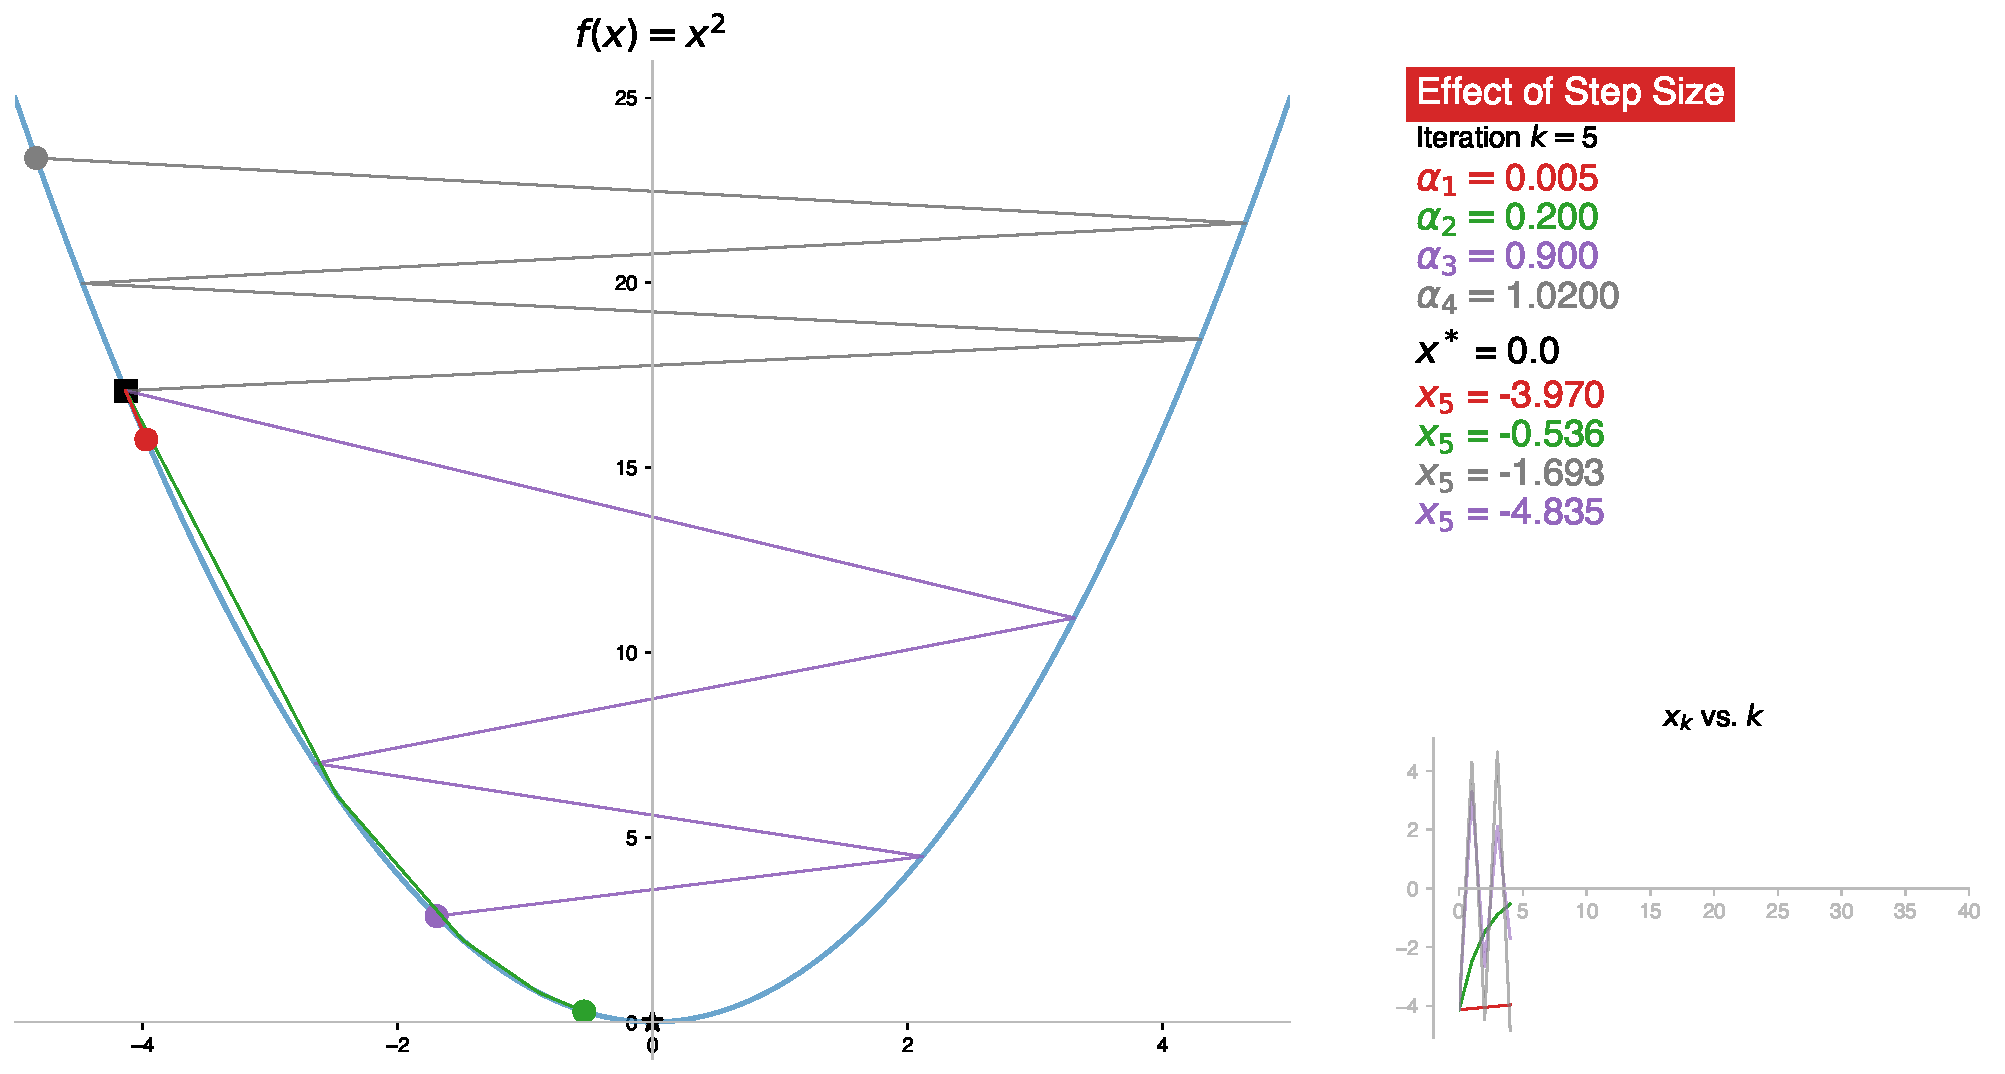
\includegraphics[width=0.8\textwidth]{figs/gd_stepsize.pdf}
  \end{figure}
\end{frame}


\begin{frame}{Unconstrained Optimization: Newton's method}
  One way to address the issue with choosing an appropriate $\alpha_k$ is to make use of the local curvatute of $f$, i.e. use the second derivative.
  \vspace{0.25cm}
  
  One of the most common line search methods is the Newton's methods, which uses the first and second derivatives of the function $f$ to iteratively compute a local minimizer for a function.
  \vspace{0.25cm}
  
  At any given iteration $k$, the Newton's method uses $f\ct{x_k}$, $f'\ct{k}$, and $f''\ct{x_k}$ to fit a quadratic approximation of the function as the following,
  \[ q\ct{x} = f\ct{x_k} + f'\ct{x_k}\ct{x - x_k} + \frac{1}{2}f''\ct{x_k}\ct{x - x_k}^2 \]

  We  mininmize quadratic this approximiation $q\ct{x}$ to find the next guess $x_{k+1}$. By settinng, $q'\ct{x} = f1\ct{x_k} + f''\ct{x - x_k} = 0$, we get the next guess as,
  \[ x_{k+1} = x_k - \frac{f`\ct{x_k}'}{f''\ct{x_k}}, \quad \ct{\text{Note: } \alpha_k = \frac{1}{f''\ct{x_k}}} \]
\end{frame}


\begin{frame}{Unconstrained Optimization: Secant method}
  What if we did not have access to the $f''$? We can use an approximation for $f''$ instead, which gives us the Secant method for line search.
  \vspace{0.25cm}

  \textbf{$f'$ is unknown}: We can use $f'$ to approximate $f''$ as the following,
  \[ \hat{f}''\ct{x_k} = \frac{f'\ct{x_k} - f'\ct{x_{k-1}}}{x_k - x{_k-1}} \] 
  Using this approximation in the Newton's method and simplifying the expression, we get
  \[ x_{k+1} = \frac{f'\ct{x_k}x_{k-1} - f'\ct{x_{k-1}}x_k}{f'\ct{x_k} - f'\ct{x_{k - 1}}} \]

  It left as an exercise to shown that $x_{k+1}$ is the minimizer of the quadratic approximation of the function $f$ at the point $x_k$.

\end{frame}


\begin{frame}{Unconstrained Optimization: Secant method}
  Both the Newton's and Secant methods are examples of \textit{quadratic fit} methods. 
  \vspace{0.25cm}
  
  A third possible method foregoes the requirement of the first derivative $f'$ and use only the value of the function at three points to fit a quadratic approximation. 
  \vspace{0.25cm}

  The derivation of the iteration rule for this method is left as an exercise.
\end{frame}


\begin{frame}{Unconstrained Optimization: Newton's method}
  \textbf{When do the Newton's or the Secant method fail?} When $f''\ct{x_k} \leq 0$.
  \[ x_{k+1} = x_k - \frac{f`\ct{x_k}'}{f''\ct{x_k}} \]
  \begin{itemize}
    \item $f''\ct{x_k} \approx 0$: Step size becomes large.
    \item $f''\ct{x_k} < 0$: Step size changes sign.
  \end{itemize}
  
  One simple way to address this is to never let the demoninator become too small or negative. This can be achieved by adding a small positive number to the denominator,
  \[ x_{k+1} = x_k - \frac{f'\ct{x_k}}{f''\ct{x_k} + \lambda}, \quad \lambda > 0 \]
  The parameter $\lambda$ is called the \textit{damping parameter}.  
\end{frame}


\begin{frame}{Unconstrained Optimization: Newton's method}
  \begin{figure}
    \centering
    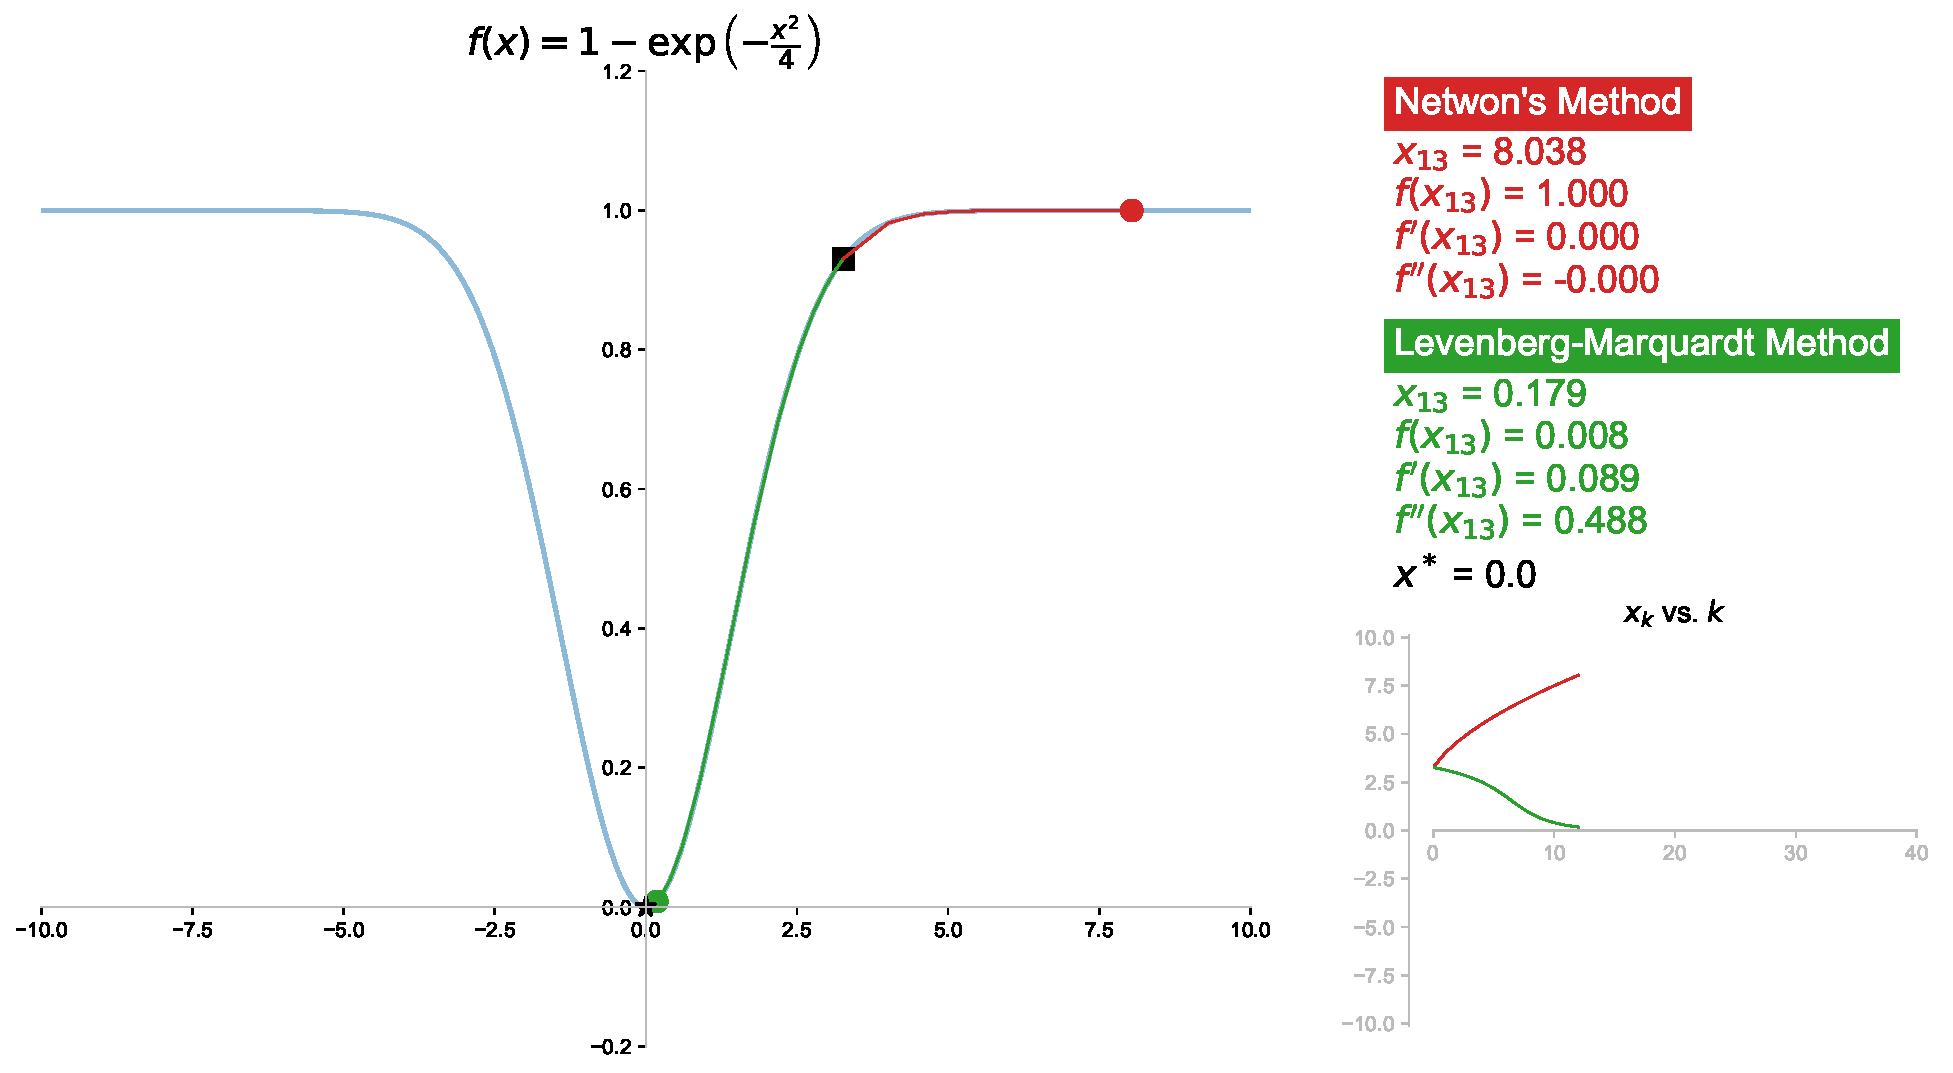
\includegraphics[width=0.8\textwidth]{figs/newton_lm_compare.pdf}
  \end{figure}
\end{frame}


\begin{frame}{Multivariate Unconstrained Optimization}
  We need to make two decisions in the multivariate case,
  \begin{itemize}
    \item The search direction $\mf{d}_k$.
    \item The step size $\alpha_k$.
  \end{itemize}
  \vspace{0.2cm}
  
  Once a search direction $\mf{d}_k$ is chosen at each iteration step, then the problem is equivalent to the univariate case. 
  \vspace{0.2cm}

  We search along that line in the direction $\mf{d}_k$. This is often called the \textit{line search} method.
  \vspace{0.2cm}

  Iterative methods for multivariate optimization are of the following form,
  \[ \mf{x}_{k+1} = \mf{x}_{k} + \alpha_k \mf{d}_{k} \]
  where, $\mf{d}_k \in \mb{R}^n$ is the search direction, and $\alpha_k$ is the step size.
  \vspace{0.2cm}

  $\mf{d}_k$ is chosen based on the local information of the function $f$ at the point $\mf{x}_k$. We choose a search direction that will lead to a decrease in the value of the function $f$.
\end{frame}


\begin{frame}{Multivariate Unconstrained Optimization}
  \begin{figure}
    \centering
    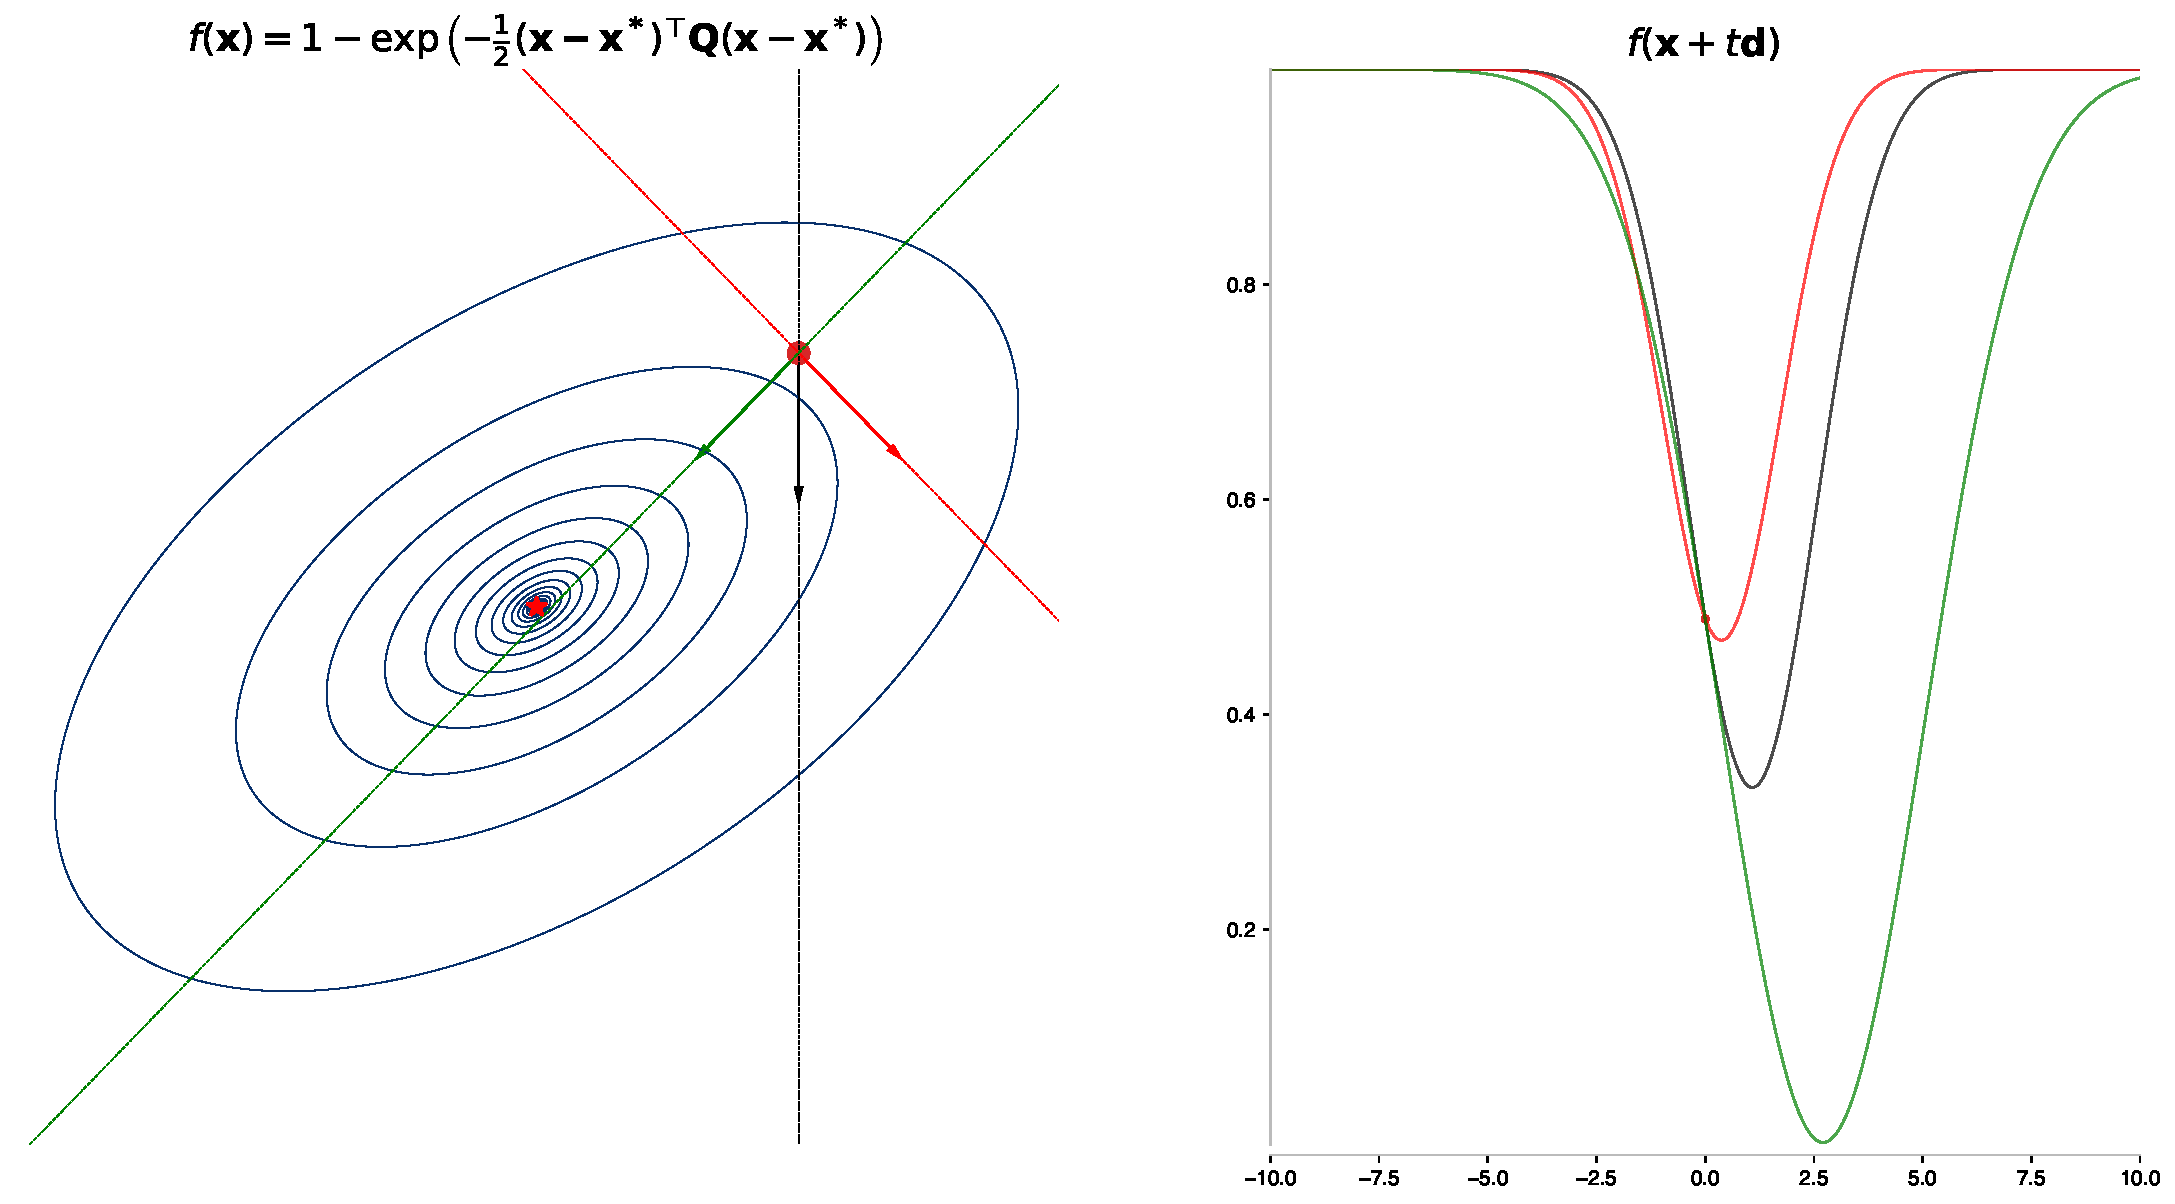
\includegraphics[width=0.85\textwidth]{figs/multivar_linesearch_demo.pdf}
  \end{figure}
\end{frame}


\begin{frame} {Multivariate Unconstrained Optimization}
  \begin{columns}
    \column{0.45\textwidth}
    The line search algorithm is shown in the figure.
    \[ \mf{x}_{k+1} = \mf{x}_{k} + \alpha_k \mf{d}_{k} \]
    The arrow indicates that change $\alpha_k \mf{d}_k$.

    Choosing $\alpha_k$ is a critical step and is often posed as a one-dimensional optimization problem at each iteration $k$,
    \[ \alpha_k^* = \arg \min_{\alpha_k \in \R_{\geq 0}} f\ct{\mf{x}_k  +\alpha_k \mf{d}_k} \]

    An ``exact line search'' will attempt to solve for $\alpha_k^*$. But this is not necessary in practice.
    \column{0.5\textwidth}
    \begin{figure}
      \centering
      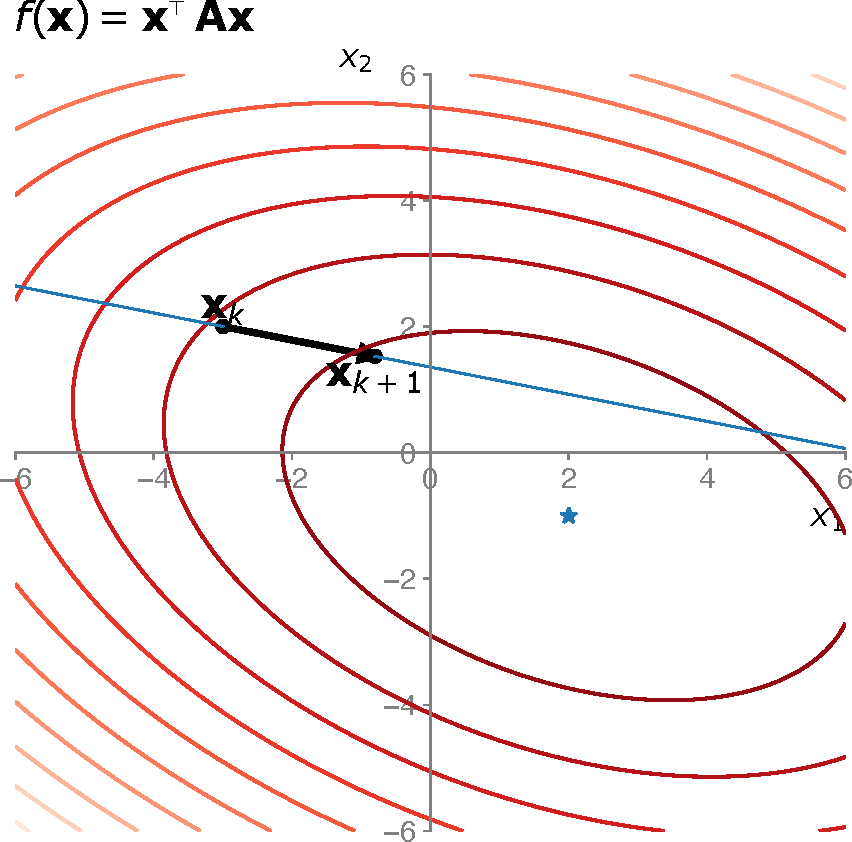
\includegraphics[width=0.9\textwidth]{figs/multivar_linesearch.pdf}
    \end{figure}
  \end{columns}
\end{frame}


\begin{frame} {Multivariate Unconstrained Optimization} 
  Inexact line searches are used in practice and with more focus on the original objective of minimizing $f\ct{\mf{x}}$.
  \vspace{0.25cm}
  
  Let $\phi_k\ct{\alpha_k} = f\ct{\mf{x}_k + \alpha_k \mf{d}_k}$.
  \textbf{Backtracking algorithm}
  \begin{enumerate}[(1)]
    \item Given $\mf{x}_k, \mf{d}_k, \alpha_{init}$.
    \item Initialize $\alpha^{\ct{0}} = \alpha_{init}$ and $l = 0$.
    \item Until $\phi\ct{\alpha^{l}} \leq \phi\ct{0}$
      \begin{enumerate}[(i)]
        \item Set $\alpha^{\ct{l+1}} = \tau \alpha^{\ct{l}}$, where $\tau \in \ct{0, 1}$ is fixed $\ct{\tau = \frac{1}{2}}$.
        \item $l = l + 1$
      \end{enumerate}
    \item Set $\alpha_k = \alpha^{\ct{l}}$.
  \end{enumerate}

  This algorithm prevents the step size from becoming too small, but does not prevent it from becoming too large.
\end{frame}


\begin{frame} {Multivariate Unconstrained Optimization} 
  A  commonly used condition is the \textit{Armijo-Goldstein} condition, which ensures that the step size $\alpha_k$ is neihter too large nor too small.
  \vspace{0.2cm}

  \textbf{Ensure $\alpha_k$ is not too large}: Let $\epsilon \in \ct{0, 1}$ and $\eta \in \ct{\epsilon, 1}$,
  \[ \text{Condition 1}: \phi_k\ct{\alpha_k} \leq \phi_k\ct{0} + \epsilon \alpha_k \phi'\ct{0} \]

  \textbf{Ensure $\alpha_k$ is not too small}
  \[ \text{Condition 2}: \phi_k\ct{\alpha_k} \geq \phi_k\ct{0} + \eta \alpha_k \phi_k'\ct{0} \]
\end{frame}


\begin{frame} {Multivariate Unconstrained Optimization} 
  \textbf{Armijo backtracking algorithm}
  \begin{enumerate}[(1)]
    \item Given $\mf{x}_k, \mf{d}_k, \alpha_{init}$.
    \item Initialize $\alpha^{\ct{0}} = \alpha_{init}$, $l = 0$, and $\epsilon \in \ct{0, 1}$.
    \item Until $\phi\ct{\alpha^{l}} \leq \phi\ct{0} + \epsilon \alpha^{l} \phi'\ct{0}$
      \begin{enumerate}[(i)]
        \item Set $\alpha^{\ct{l+1}} = \tau \alpha^{\ct{l}}$, where $\tau \in \ct{0, 1}$ is fixed $\ct{\tau = \frac{1}{2}}$.
        \item $l = l + 1$
      \end{enumerate}
    \item Set $\alpha_k = \alpha^{\ct{l}}$.
  \end{enumerate}

  This alorithm prevents the step size from becoming too small, but does not prevent it from becoming too large.
\end{frame}


\begin{frame} {Multivariate Unconstrained Optimization}
  Consider the function $f: \R^n \to \R$ and $\mf{x} \in \R^n$.
  \vspace{0.25cm}

  The best search direction $\mf{d}_k$ at at the point $\mf{x}_k$ is the direction that maximally minimizes the value of the function $f$ at the point $\mf{x}_k$.
  \vspace{0.25cm}

  The directional derivative of the function $f\ct{\mf{x}}$ at the point $\mf{x}$ along the direction $\mf{d}$ is defined as,
  \[ \lim_{\alpha \to 0} \frac{f\ct{\mf{x} + \alpha \mf{d}} - f\ct{\mf{x}}}{\alpha} = \mf{d}^\top \nabla_{\mf{x}^\top} f\ct{\mf{x}} \]
  We will use $\nabla f\ct{\mf{x}}$ to denote $\nabla_{\mf{x}^\top} f\ct{\mf{x}}$ from this point foward.

  \[ \Vert \mf{d} \Vert_2 = 1 \implies \mf{d}^\top \nabla f\ct{\mf{x}} \leq \Vert \nabla f\ct{\mf{x}} \Vert \implies \mf{d} = \frac{\nabla f\ct{\mf{x}}}{\Vert \nabla f\ct{\mf{x}} \Vert} \]

  Thus, we have,
  \[ f\ct{\mf{x}_k - \alpha \nabla f\ct{\mf{x}_k}} =  f\ct{\mf{x}_k} - \alpha \Vert \nabla f\ct{\mf{x}_k} \Vert_2^2 + o\ct{\alpha} \]
\end{frame}


\begin{frame} {Multivariate Unconstrained Optimization}
  Thus, we have,
  \[ f\ct{\mf{x}_k - \alpha \nabla f\ct{\mf{x}_k}} =  f\ct{\mf{x}_k} - \alpha \Vert \nabla f\ct{\mf{x}_k} \Vert_2^2 + o\ct{\alpha} \]

  For a small enough value for $\alpha > 0$, we have,
  \[ f\ct{\mf{x}_k - \alpha \nabla f\ct{\mf{x}_k}} < f\ct{\mf{x}_k} \]

  Thus, the movement along the direction of the negative gradient of the function $f$ at the point $\mf{x}_k$ will lead to a decrease in the value of the function $f$.
\end{frame}


\begin{frame} {Multivariate Unconstrained Optimization: Gradient descent}
  The gradient descent algorithm with a fixed step size can be used for minimizing the function $f\ct{\mf{x}}$.
  \[ \mf{x}_{k+1} = \mf{x}_{k} - \alpha \nabla f\ct{\mf{x}_k} \]
  The value of $\alpha$ is a simple approach, but runs into similar problem as in the single variable case. 
  \vspace{0.2cm}
  
  The above equation can be thought of as $n$ separate single variable optimization problems, and a fixed $\alpha$ might is unlikely to be the best choice for all of them. The $i^{th}$ component of the vector $\mf{x}_k$ will be updated as,
  \[ x_{{k+1}, i} = x_{{k}, i} - \alpha \frac{\partial f}{\partial x_i}\ct{\mf{x}_k} \]
  where $\mf{x}_k = \bmx x_{k, 1} & x_{k, 2} & \cdots & x_{k, n}\emx^\top$.
\end{frame}


\begin{frame} {Multivariate Unconstrained Optimization: Gradient descent}
  Just as in the single variable case, an appropriate choice of $\alpha$ will depend on the curvature of the function $f\ct{\mf{x}}$, which is given by the Hessian matrix $\mf{H}\ct{\mf{x}}$.
  \vspace{0.2cm}

  For a quadratic function $f\ct{\mf{x}} = \frac{1}{2}\mf{x}^\top \mf{H} \mf{x} + \mf{b}^\top \mf{x} + c$, the following choice for the step size will ensure convergence of $\mf{x}_k$ to the minimizer of the function $f\ct{\mf{x}}$.
  \[ 0 < \alpha < \frac{2}{\lambda_{max}\ct{\mf{H}}}, \,\, \mf{H} \geq 0 \]
  where, $\lambda_{max}\ct{\mf{H}}$ is the largest eigenvalue of the Hessian matrix $\mf{H}$.
\end{frame}

\end{document}